% generated from JIRA project LVV
% using template at /usr/share/miniconda/envs/docsteady-env/lib/python3.11/site-packages/docsteady/templates/tpr.latex.jinja2.
% using docsteady version 0.0.0
% Please do not edit -- update information in Jira instead
\documentclass[DM,lsstdraft,STR,toc]{lsstdoc}
\usepackage{geometry}
\usepackage{longtable,booktabs}
\usepackage{enumitem}
\usepackage{arydshln}
\usepackage{attachfile}
\usepackage{array}
\usepackage{dashrule}
\usepackage{pdfpages}

\newcolumntype{L}[1]{>{\raggedright\let\newline\\\arraybackslash\hspace{0pt}}p{#1}}

\input{meta.tex}

\newcommand{\attachmentsUrl}{https://github.com/\gitorg/\lsstDocType-\lsstDocNum/blob/\gitref/attachments}
\providecommand{\tightlist}{
  \setlength{\itemsep}{0pt}\setlength{\parskip}{0pt}}

\setcounter{tocdepth}{4}

\providecommand{\ul}[1]{\textbf{#1}}

\begin{document}

\def\milestoneName{Replication of Summit EFD to USDF}
\def\milestoneId{LDM-503-EFDb}
\def\product{Data Management}

\setDocCompact{true}

\title{LDM-503-EFDb: Replication of Summit EFD to USDF Test Plan and Report}
\setDocRef{\lsstDocType-\lsstDocNum}
\date{ 2023-09-03 }
\author{ Wil O'Mullane }

% Most recent last
\setDocChangeRecord{
\addtohist{}{2021-10-19}{First draft}{K. Simon Krughoff}
}

\setDocCurator{K. Simon Krughoff}
\setDocUpstreamLocation{\url{https://github.com/lsst-dm/\lsstDocType-\lsstDocNum}}
\setDocUpstreamVersion{\vcsRevision}



\setDocAbstract{
This is the test plan and report for
\textbf{ Replication of Summit EFD to USDF} (LDM-503-EFDb),
an LSST milestone pertaining to the Data Management Subsystem.\\
This document is based on content automatically extracted from the Jira test database on \docDate.
The most recent change to the document repository was on \vcsDate.
}


\maketitle

\section{Introduction}
\label{sect:intro}


\subsection{Objectives}
\label{sect:objectives}

 The purpose of this test plan is to describe all the necessary
requirements and infrastructure for successfully testing the replication
and archive of the Engineering Facility Database (EFD) as implemented
with Kafka, InfluxDB and Chronograf from the summit to the USDF. This
plan will describe the prerequisites for beginning a test campaign, step
by step instructions for each test case and a description of the
expected results and test artifacts.\\
\strut \\
NB: The use of the term reliability in this document is intended to
indicate the number of messages produced relative to the number of
messages recorded in the EFD. The system shall be considered reliable if
at least 99.9\% of produced messages are recorded.\\
\strut \\
At a high level, this test plan is intended to show that a nominally
operating EFD at the summit is able to be replicated to the USDF and
archived for future use either directly or via ingest into a secondary
database management technology. We assume here that the archive
technology will be parquet datasets stored on persistent/redundant disk
at the USDF. There are no latency requirements in this test plan, but we
will show that the replication and archiving are not falling behind
relative to the summit instance in the aggregate. We choose a period of
6 days of continuous nominal operation in order to test the cases in
this test plan.\\
Successful completion of the test campaign will show that:\\

\begin{enumerate}
\tightlist
\item
  users are able to access the same information at the USDF EFD that was
  originally ingested in the summit version
\item
  the reliability of the replication is better than the minimum of 99\%
\item
  archive products are able to be used as a primary source of
  information for historical examination of EFD topics
\end{enumerate}



\subsection{System Overview}
\label{sect:systemoverview}

 The tests will be carried out from within an instance of the notebook
aspect of the RSP running at the data facility where the EFD replication
is currently happening. An appropriate weekly version of the stack will
be chosen.


\subsection{Document Overview}
\label{sect:docoverview}

This document was generated from Jira, obtaining the relevant information from the
\href{https://jira.lsstcorp.org/secure/Tests.jspa\#/testPlan/LVV-P90}{LVV-P90}
~Jira Test Plan and related Test Cycles (
\href{https://jira.lsstcorp.org/secure/Tests.jspa\#/testCycle/LVV-C181}{LVV-C181}
).

Section \ref{sect:intro} provides an overview of the test campaign, the system under test (\product{}),
the applicable documentation, and explains how this document is organized.
Section \ref{sect:testplan} provides additional information about the test plan, like for example the configuration
used for this test or related documentation.
Section \ref{sect:personnel} describes the necessary roles and lists the individuals assigned to them.

Section \ref{sect:overview} provides a summary of the test results, including an overview in Table \ref{table:summary},
an overall assessment statement and suggestions for possible improvements.
Section \ref{sect:detailedtestresults} provides detailed results for each step in each test case.

The current status of test plan \href{https://jira.lsstcorp.org/secure/Tests.jspa\#/testPlan/LVV-P90}{LVV-P90} in Jira is \textbf{ Approved }.

\subsection{References}
\label{sect:references}
\renewcommand{\refname}{}
\bibliography{lsst,refs,books,refs_ads,local}


\newpage
\section{Test Plan Details}
\label{sect:testplan}


\subsection{Data Collection}

  Observing is not required for this test campaign.

\subsection{Verification Environment}
\label{sect:hwconf}
  The environment will be within notebooks running a modern stack.

  \subsection{Entry Criteria}
  \begin{enumerate}
\tightlist
\item
  Before beginning this test, a set of viability tests shall be
  performed. These will show:

  \begin{enumerate}
  \tightlist
  \item
    The system demonstrates reliability (number of recorded
    messages/number of produced messages) of greater than 99.9\%
  \item
    The summit data is being replicated to the instance at USDF
  \item
    Chronograf is set up and running at both the summit and USDF
  \end{enumerate}
\item
  The summit network and Kubernetes cluster are performing nominally
\item
  A number of telemetry topics are reliably producing telemetry at both
  low frequency (1 Hz) and high frequency (\textgreater{} 10 Hz).
\item
  The notebook aspect of the RSP is deployed in the summit Kubernetes
  cluster
\item
  The summit EFD is reliably replicated to an EFD instance running in a
  data facility
\item
  The notebook aspect of the RSP is deployed in the same data facility
  as that running the replicated EFD
\item
  The most recent version of the EFD client python modules are installed
  in the various deployed notebook aspects
\item
  The replication system is also successfully archiving EFD topics to
  parquet files on persistent disk at the data facility
\end{enumerate}



\subsection{Related Documentation}


No additional documentation provided.


\subsection{PMCS Activity}

Primavera milestones related to the test campaign:
\begin{itemize}
\item LDM-503-EFDb
\end{itemize}


\newpage
\section{Personnel}
\label{sect:personnel}

The personnel involved in the test campaign is shown in the following table.

{\small
\begin{longtable}{p{3cm}p{3cm}p{3cm}p{6cm}}
\hline
\multicolumn{2}{r}{T. Plan \href{https://jira.lsstcorp.org/secure/Tests.jspa\#/testPlan/LVV-P90}{LVV-P90} owner:} &
\multicolumn{2}{l}{\textbf{ Wil O'Mullane } }\\\hline
\multicolumn{2}{r}{T. Cycle \href{https://jira.lsstcorp.org/secure/Tests.jspa\#/testCycle/LVV-C181}{LVV-C181} owner:} &
\multicolumn{2}{l}{\textbf{
Wil O'Mullane }
} \\\hline
\textbf{Test Cases} & \textbf{Assigned to} & \textbf{Executed by} & \textbf{Additional Test Personnel} \\ \hline
\href{https://jira.lsstcorp.org/secure/Tests.jspa#/testCase/LVV-T2338}{LVV-T2338}
& {\small Wil O'Mullane } & {\small Wil O'Mullane } &
\begin{minipage}[]{6cm}
\smallskip
{\small  }
\medskip
\end{minipage}
\\ \hline
\href{https://jira.lsstcorp.org/secure/Tests.jspa#/testCase/LVV-T2339}{LVV-T2339}
& {\small Wil O'Mullane } & {\small Wil O'Mullane } &
\begin{minipage}[]{6cm}
\smallskip
{\small William O\textquotesingle Mullane\\
\strut \\ }
\medskip
\end{minipage}
\\ \hline
\end{longtable}
}

\newpage

\section{Test Campaign Overview}
\label{sect:overview}

\subsection{Summary}
\label{sect:summarytable}

{\small
\begin{longtable}{p{2cm}cp{2.3cm}p{8.6cm}p{2.3cm}}
\toprule
\multicolumn{2}{r}{ T. Plan \href{https://jira.lsstcorp.org/secure/Tests.jspa\#/testPlan/LVV-P90}{LVV-P90}:} &
\multicolumn{2}{p{10.9cm}}{\textbf{ LDM-503-EFDb: Replication of Summit EFD to USDF }} & Approved \\\hline
\multicolumn{2}{r}{ T. Cycle \href{https://jira.lsstcorp.org/secure/Tests.jspa\#/testCycle/LVV-C181}{LVV-C181}:} &
\multicolumn{2}{p{10.9cm}}{\textbf{ LDM-503-EFDb: Replication of Summit EFD to USDF }} & Done \\\hline
\textbf{Test Cases} &  \textbf{Ver.} & \textbf{Status} & \textbf{Comment} & \textbf{Issues} \\\toprule
\href{https://jira.lsstcorp.org/secure/Tests.jspa#/testCase/LVV-T2338}{LVV-T2338}
&  2
& Fail &
\begin{minipage}[]{9cm}
\smallskip

\medskip
\end{minipage}
&   \\\hline
\href{https://jira.lsstcorp.org/secure/Tests.jspa#/testCase/LVV-T2339}{LVV-T2339}
&  3
& Pass &
\begin{minipage}[]{9cm}
\smallskip

\medskip
\end{minipage}
&   \\\hline
\caption{Test Campaign Summary}
\label{table:summary}
\end{longtable}
}

\subsection{Overall Assessment}
\label{sect:overallassessment}

Not yet available.

\subsection{Recommended Improvements}
\label{sect:recommendations}

Not yet available.

\newpage
\section{Detailed Test Results}
\label{sect:detailedtestresults}

\subsection{Test Cycle LVV-C181 }

Open test cycle {\it \href{https://jira.lsstcorp.org/secure/Tests.jspa#/testrun/LVV-C181}{LDM-503-EFDb: Replication of Summit EFD to USDF}} in Jira.

Test Cycle name: LDM-503-EFDb: Replication of Summit EFD to USDF\\
Status: Done



\subsubsection{Software Version/Baseline}
Not provided.

\subsubsection{Configuration}
Not provided.

\subsubsection{Test Cases in LVV-C181 Test Cycle}

\paragraph{ LVV-T2338 - Replicated telemetry data agrees with telemetry produced at the summit }\mbox{}\\

Version \textbf{2}.
Status \textbf{Approved}.
Open  \href{https://jira.lsstcorp.org/secure/Tests.jspa#/testCase/LVV-T2338}{\textit{ LVV-T2338 } }
test case in Jira.

Show that telemetry data can be accessed from the replicated EFD.
~Further, show that the values in the replicated database agree with the
values in the summit EFD over a specified time range and set of
topics.\\
\strut \\
This test case provides partial coverage of the requirement
DMS-REQ-0168, Summit Facility Data Communications: "The DMS shall
provide data communications infrastructure to accept science data and
associated metadata read-outs, and \textbf{the collection of ancillary
and engineering data}, for transfer to the base facility.", as adapted
to the current design for EFD replication (see
\href{https://dmtn-082.lsst.io}{DMTN-082}).

\textbf{ Preconditions}:\\
See prerequisites in the Test Plan LVV-P90

Execution status: {\bf Fail }

Final comment:\\


Detailed steps results:

\begin{tabular}{p{2cm}p{14cm}}
\toprule
Step 1 & Step Execution Status: \textbf{ Pass } \\ \hline
\end{tabular}
 Description \\
{\footnotesize
Log in to the USDF notebook aspect:
https://usdf-rsp-dev.slac.stanford.edu/\\
Make sure to choose a recent weekly release and a large instance; record
the chosen release and whether or not it is the current "recommended"
release.

}
\hdashrule[0.5ex]{\textwidth}{1pt}{3mm}
  Expected Result \\
{\footnotesize
The JupyterLab interface is displayed in the browser

}
\hdashrule[0.5ex]{\textwidth}{1pt}{3mm}
  Actual Result \\
{\footnotesize
Logged in choose large with latest weekly (23)

}
\begin{tabular}{p{2cm}p{14cm}}
\toprule
Step 2 & Step Execution Status: \textbf{ Pass } \\ \hline
\end{tabular}
 Description \\
{\footnotesize
Open a notebook:

\begin{enumerate}
\tightlist
\item
  Navigate to the File-\textgreater New-\textgreater Notebook
\item
  When prompted, select the LSST kernel
\end{enumerate}

}
\hdashrule[0.5ex]{\textwidth}{1pt}{3mm}
  Expected Result \\
{\footnotesize
An empty notebook running in the LSST kernel

}
\hdashrule[0.5ex]{\textwidth}{1pt}{3mm}
  Actual Result \\
{\footnotesize
Created a notebook LVV-T2338

}
\begin{tabular}{p{2cm}p{14cm}}
\toprule
Step 3 & Step Execution Status: \textbf{ Pass } \\ \hline
\end{tabular}
 Description \\
{\footnotesize
Connect to the USDF EFD.\\
Use the EFD identifier name from the test case parameter,
{ldf\_stable\_efd}⁠ , unless it is necessary to change at the time the
test is executed. ~Record the value used if different.

}
\hdashrule[0.5ex]{\textwidth}{1pt}{3mm}
  Example Code \\
{\footnotesize
from lsst\_efd\_client import EfdClient\\
efd = EfdClient(\textquotesingle usdf\_efd\textquotesingle)

}
\hdashrule[0.5ex]{\textwidth}{1pt}{3mm}
  Expected Result \\
{\footnotesize
A notebook with an instance of the `EfdClient` configured to talk to the
NCSA EFD

}
\hdashrule[0.5ex]{\textwidth}{1pt}{3mm}
  Actual Result \\
{\footnotesize
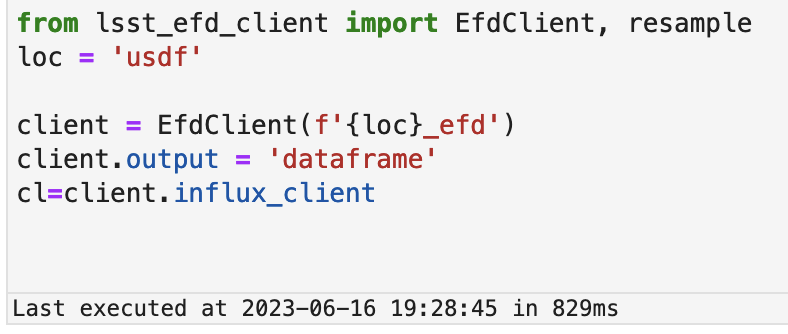
\includegraphics[width=3.125in, ]{jira_imgs/3911.png}

}
\begin{tabular}{p{2cm}p{14cm}}
\toprule
Step 4 & Step Execution Status: \textbf{ Pass } \\ \hline
\end{tabular}
 Description \\
{\footnotesize
Since we need to compare results between the summit and the USDF, also
create a connection to the summit EFD. ~Use the EFD identifier name from
the test case parameter, {summit\_efd}⁠ , unless it is necessary to
change at the time the test is executed. ~Record the value used if
different.

}
\hdashrule[0.5ex]{\textwidth}{1pt}{3mm}
  Example Code \\
{\footnotesize
efd\_summit = EfdClient(\textquotesingle summit\_efd\textquotesingle)

}
\hdashrule[0.5ex]{\textwidth}{1pt}{3mm}
  Expected Result \\
{\footnotesize
Another cell in the notebook with a second EFD connection to the summit
EFD

}
\hdashrule[0.5ex]{\textwidth}{1pt}{3mm}
  Actual Result \\
{\footnotesize
times out - you can not access efd\_summit from USDF.\\
Connected to https://summit-lsp.lsst.codes/nb this allows connections to
both USDF and Summit EFD.

}
\begin{tabular}{p{2cm}p{14cm}}
\toprule
Step 5 & Step Execution Status: \textbf{ Pass } \\ \hline
\end{tabular}
 Description \\
{\footnotesize
Choose 5 topics to query and select a 6 day window of data. The window
is arbitrary, but must be explicit (not relative to now()) so that it
can be reproduced. The topics should be chosen to sample the various
topic contexts. I.e. the topics should be chosen to sample both
diagnostic topics like heartbeat monitors as well as both high and low
cadence telemetry topics to get a broad view on how the system behaves
with different kinds of topics.

}
\hdashrule[0.5ex]{\textwidth}{1pt}{3mm}
  Expected Result \\
{\footnotesize
A list of 5 valid SAL topics to be queried and a time window defined as
astropy.Time objects.

}
\hdashrule[0.5ex]{\textwidth}{1pt}{3mm}
  Actual Result \\
{\footnotesize
\begin{verbatim}
Random selction of five 'summit' topics ['lsst.sal.GIS.logevent_heartbeat', 'lsst.sal.ATOODS.logevent_heartbeat', 'lsst.sal.Test.logevent_heartbeat', 'lsst.sal.ESS.relativeHumidity', 'lsst.sal.ESS.logevent_heartbeat'] with messages on 2023-05-20
\end{verbatim}

}
\begin{tabular}{p{2cm}p{14cm}}
\toprule
Step 6 & Step Execution Status: \textbf{ Pass } \\ \hline
\end{tabular}
 Description \\
{\footnotesize
Issue selections at both the summit and the data facility. These
selections should select all fields for the chosen topics.

}
\hdashrule[0.5ex]{\textwidth}{1pt}{3mm}
  Expected Result \\
{\footnotesize
A total of 10 pandas.DataFrame objects, 5 each for the summit and
replicated EFDs. ~Each topic requires a separate query, so each will get
its own DataFrame. ~All fields in each topic should be selected.

}
\hdashrule[0.5ex]{\textwidth}{1pt}{3mm}
  Actual Result \\
{\footnotesize
combined with next step

}
\begin{tabular}{p{2cm}p{14cm}}
\toprule
Step 7 & Step Execution Status: \textbf{ Fail } \\ \hline
\end{tabular}
 Description \\
{\footnotesize
First compare the index for each topic between the summit and replicated
EFD. ~There should be:\\

\begin{enumerate}
\tightlist
\item
  The same number of samples in each topic for each location
\item
  Given 1) each time stamp should represent the same time
\end{enumerate}

Reliability of the replication must be at better than 99\%. If there are
samples missing from the replicated datasets, confirm that the length of
the replicated DataFrame divided by the length of the summit DataFrame
is greater than 0.99 for all topics.

}
\hdashrule[0.5ex]{\textwidth}{1pt}{3mm}
  Expected Result \\
{\footnotesize
A cell in the notebook showing the DataFrames are the same length per
topic between the summit and the replicated EFD. ~A cell showing the
times in the index are the same for each topic. ~This could be done by
converting to seconds and showing the difference is zero for every
sample.\\
\strut \\
If there are missing samples, the replication should be better than
99\%. ~If it is not, the deviation must be traced to an intervening
event or system other than the replication system itself to explain the
discrepancy.

}
\hdashrule[0.5ex]{\textwidth}{1pt}{3mm}
  Actual Result \\
{\footnotesize
\begin{verbatim}
lsst.sal.GIS.logevent_heartbeat had 189633 messages - summit had 189615
lsst.sal.GIS.logevent_heartbeat does not match
lsst.sal.ATOODS.logevent_heartbeat had 186155 messages - summit had 186148
lsst.sal.ATOODS.logevent_heartbeat does not match
lsst.sal.Test.logevent_heartbeat had 188501 messages - summit had 188484
lsst.sal.Test.logevent_heartbeat does not match
lsst.sal.ESS.relativeHumidity had 528737 messages - summit had 528478
lsst.sal.ESS.relativeHumidity does not match
\end{verbatim}

}
\begin{tabular}{p{2cm}p{14cm}}
\toprule
Step 8 & Step Execution Status: \textbf{ Blocked } \\ \hline
\end{tabular}
 Description \\
{\footnotesize
Compare the fields for each topic between the summit and the replicated
EFDs. ~They should be equivalent to double precision. ~This can be done
by looping over the topics and fields and showing numpy.all (or similar)
evaluates to True.

}
\hdashrule[0.5ex]{\textwidth}{1pt}{3mm}
  Expected Result \\
{\footnotesize
A cell or cells showing that all fields for all topics evaluate as
equivalent given appropriate precision.

}
\hdashrule[0.5ex]{\textwidth}{1pt}{3mm}
  Actual Result \\
{\footnotesize

}
\begin{tabular}{p{2cm}p{14cm}}
\toprule
Step 9 & Step Execution Status: \textbf{ Pass } \\ \hline
\end{tabular}
 Description \\
{\footnotesize
Examine the summit messages to confirm that the reliability is better
than 99.9\% for all topics. ~Keep in mind that the private\_seqNum is
intended to be a sequentially increasing index of the messages, but that
it gets reset after every CSC reboot. ~This must be accounted for by
applying an offset when a reset is observed.\\
Show the reliability is better than 99.9\% by showing that the
private\_seqNum is sequential better than 99.9\% of the time (when
correcte for resets).

}
\hdashrule[0.5ex]{\textwidth}{1pt}{3mm}
  Expected Result \\
{\footnotesize
A histogram or similar showing that the difference
private\_seqNum{[}1:{]} - private\_seqnum{[}:-1{]} is 1 more than 99.9\%
of the time.

}
\hdashrule[0.5ex]{\textwidth}{1pt}{3mm}
  Actual Result \\
{\footnotesize
\begin{verbatim}
lsst.sal.GIS.logevent_heartbeat private_seqNum increases 100.0% of the sequence
lsst.sal.ATOODS.logevent_heartbeat private_seqNum increases 100.0% of the sequence
lsst.sal.Test.logevent_heartbeat private_seqNum increases 100.0% of the sequence
lsst.sal.ESS.relativeHumidity private_seqNum increases 100.0% of the sequence
lsst.sal.ESS.logevent_heartbeat private_seqNum increases 100.0% of the sequence
\end{verbatim}

}
\begin{tabular}{p{2cm}p{14cm}}
\toprule
Step 10 & Step Execution Status: \textbf{ Pass } \\ \hline
\end{tabular}
 Description \\
{\footnotesize
Document the procedure including topics chosen, time window, replication
reliability and EFD reliability

}
\hdashrule[0.5ex]{\textwidth}{1pt}{3mm}
  Expected Result \\
{\footnotesize
\begin{itemize}
\tightlist
\item
  A document describing the process including topics and time window.
\item
  The document shall be in the form of a notebook with saved outputs, or
  similar
\end{itemize}

}
\hdashrule[0.5ex]{\textwidth}{1pt}{3mm}
  Actual Result \\
{\footnotesize
Added LVV-T2334.ipynb to the test report repo

}

\paragraph{ LVV-T2339 - Archival EFD products can be used for historical analysis }\mbox{}\\

Version \textbf{3}.
Status \textbf{Approved}.
Open  \href{https://jira.lsstcorp.org/secure/Tests.jspa#/testCase/LVV-T2339}{\textit{ LVV-T2339 } }
test case in Jira.

Show that the archival replicated EFD products (nominally Parquet files)
can be used to query for topics post facto and that analysis in the
Notebook Aspect of the RSP is not only possible but straightforward.\\
\strut \\
This test case provides partial coverage of the requirement
DMS-NB-REQ-0023, Access to All Data Products: "An authorized user of the
Notebook Aspect shall be able to access the Transformed Engineering and
Facilities Database (EFD) and and all other LSST released data
products.", as adapted to the current design for EFD replication and
access (see \href{https://dmtn-082.lsst.io}{DMTN-082}). ~Note that it is
still also anticipated that TAP access to the EFD will be provided in
the RSP as an alternative to the Python-API access covered by this test
case. ~Note in particular that this test case does not cover the feature
of the "Transformed" EFD from the original design in which EFD data is
pre-processed with associations to exposure/visit IDs.

\textbf{ Preconditions}:\\


Execution status: {\bf Pass }

Final comment:\\


Detailed steps results:

\begin{tabular}{p{2cm}p{14cm}}
\toprule
Step 1 & Step Execution Status: \textbf{ Pass } \\ \hline
\end{tabular}
 Description \\
{\footnotesize
Log in to the USDF notebook aspect:
https://usdf-rsp-dev.slac.stanford.edu/\\
Make sure to choose a recent weekly release and a large instance; record
the chosen release and whether or not it is the current "recommended"
release.

}
\hdashrule[0.5ex]{\textwidth}{1pt}{3mm}
  Expected Result \\
{\footnotesize
The JupyterLab interface is displayed in the browser

}
\hdashrule[0.5ex]{\textwidth}{1pt}{3mm}
  Actual Result \\
{\footnotesize
logged in have RSP at USDF

}
\begin{tabular}{p{2cm}p{14cm}}
\toprule
Step 2 & Step Execution Status: \textbf{ Pass } \\ \hline
\end{tabular}
 Description \\
{\footnotesize
Open a notebook:

\begin{enumerate}
\tightlist
\item
  Navigate to the File-\textgreater New-\textgreater Notebook
\item
  When prompted, select the LSST kernel
\end{enumerate}

}
\hdashrule[0.5ex]{\textwidth}{1pt}{3mm}
  Expected Result \\
{\footnotesize
An empty notebook running in the LSST kernel

}
\hdashrule[0.5ex]{\textwidth}{1pt}{3mm}
  Actual Result \\
{\footnotesize
Copied LVV-T2338.ipynb to LVV-TT339.ipynb

}
\begin{tabular}{p{2cm}p{14cm}}
\toprule
Step 3 & Step Execution Status: \textbf{ Pass } \\ \hline
\end{tabular}
 Description \\
{\footnotesize
Connect to the USDF EFD.\\
Use the EFD identifier name from the test case parameter, {usdf\_efd}⁠ ⁠ ,
unless it is necessary to change at the time the test is executed.
~Record the value used if different.

}
\hdashrule[0.5ex]{\textwidth}{1pt}{3mm}
  Example Code \\
{\footnotesize
from lsst\_efd\_client import EfdClient\\
efd = EfdClient(\textquotesingle\{EFD\_ID\}\textquotesingle)

}
\hdashrule[0.5ex]{\textwidth}{1pt}{3mm}
  Expected Result \\
{\footnotesize
A notebook with an instance of the `EfdClient` configured to talk to the
USDF EFD

}
\hdashrule[0.5ex]{\textwidth}{1pt}{3mm}
  Actual Result \\
{\footnotesize
Last executed at 2023-06-16 19:50:41 in 3.71s

}
\begin{tabular}{p{2cm}p{14cm}}
\toprule
Step 4 & Step Execution Status: \textbf{ Not Executed } \\ \hline
\end{tabular}
 Description \\
{\footnotesize
Choose 3 topics to query and select a 6 day window of data. The window
is arbitrary, but must be explicit (not relative to now()) so that it
can be reproduced. The topics are also arbitrary but will sample
multiple subsystems.

}
\hdashrule[0.5ex]{\textwidth}{1pt}{3mm}
  Expected Result \\
{\footnotesize
A cell in a notebook specifying topic names and start and end times for
a 6 day window as astropy.Time objects.

}
\hdashrule[0.5ex]{\textwidth}{1pt}{3mm}
  Actual Result \\
{\footnotesize
\begin{verbatim}
lsst.sal.ATPneumatics.logevent_heartbeat had 529266 messages between 2023-06-13 and 2023-06-20 
lsst.sal.MTAirCompressor.logevent_summaryState had 22 messages between 2023-06-13 and 2023-06-20 
lsst.sal.MTM1M3.logevent_raisingLoweringInfo had 6582 messages between 2023-06-13 and 2023-06-20 
Random selction of 3 'usdf' topics ['lsst.sal.ATPneumatics.logevent_heartbeat', 'lsst.sal.MTAirCompressor.logevent_summaryState', 'lsst.sal.MTM1M3.logevent_raisingLoweringInfo'] with messages between 2023-06-13 and 2023-06-20
\end{verbatim}

}
\begin{tabular}{p{2cm}p{14cm}}
\toprule
Step 5 & Step Execution Status: \textbf{ Pass } \\ \hline
\end{tabular}
 Description \\
{\footnotesize
Use the defined topics and the time window to read in fields from the
chosen topics. These are expected to be pandas.DataFrames.

}
\hdashrule[0.5ex]{\textwidth}{1pt}{3mm}
  Expected Result \\
{\footnotesize
A cell in a notebook with 1 DataFrame per topic. This shall be explicit
about all the necessary steps and any hand tuning necessary to make it
possible to make selections from the archival data.

}
\hdashrule[0.5ex]{\textwidth}{1pt}{3mm}
  Actual Result \\
{\footnotesize
\begin{verbatim}
lsst.sal.ATPneumatics.logevent_heartbeat has fields:Index(['heartbeat', 'private_efdStamp', 'private_identity',
       'private_kafkaStamp', 'private_origin', 'private_rcvStamp',
       'private_revCode', 'private_seqNum', 'private_sndStamp'],
      dtype='object')
lsst.sal.MTAirCompressor.logevent_summaryState has fields:Index(['private_efdStamp', 'private_identity', 'private_kafkaStamp',
       'private_origin', 'private_rcvStamp', 'private_revCode',
       'private_seqNum', 'private_sndStamp', 'salIndex', 'summaryState'],
      dtype='object')
lsst.sal.MTM1M3.logevent_raisingLoweringInfo has fields:Index(['private_efdStamp', 'private_identity', 'private_kafkaStamp',
       'private_origin', 'private_rcvStamp', 'private_revCode',
       'private_seqNum', 'private_sndStamp', 'waitAirPressure',
       'waitHardpoint0',
       ...
       'waitZForceActuator91', 'waitZForceActuator92', 'waitZForceActuator93',
       'waitZForceActuator94', 'waitZForceActuator95', 'waitZForceActuator96',
       'waitZForceActuator97', 'waitZForceActuator98', 'waitZForceActuator99',
       'weightSupportedPercent'],
      dtype='object', length=284)
\end{verbatim}

}
\begin{tabular}{p{2cm}p{14cm}}
\toprule
Step 6 & Step Execution Status: \textbf{ Pass } \\ \hline
\end{tabular}
 Description \\
{\footnotesize
Execute various analysis tasks, e.g. plotting various quantities, to
show that it is practical to do so.

}
\hdashrule[0.5ex]{\textwidth}{1pt}{3mm}
  Expected Result \\
{\footnotesize
Plots of quantities including filtering and other common activities.
~This shall specifically identify cases where there is an obvious
difference between how the interaction would be done with the running
EFD vs the archival version.

}
\hdashrule[0.5ex]{\textwidth}{1pt}{3mm}
  Actual Result \\
{\footnotesize
not so interesting plots like this\\
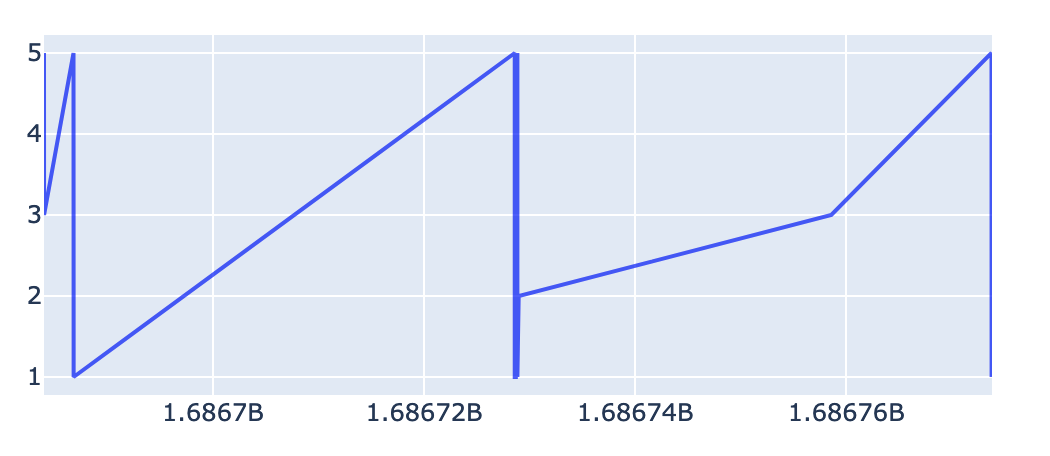
\includegraphics[width=3.125in, ]{jira_imgs/3922.png}\\
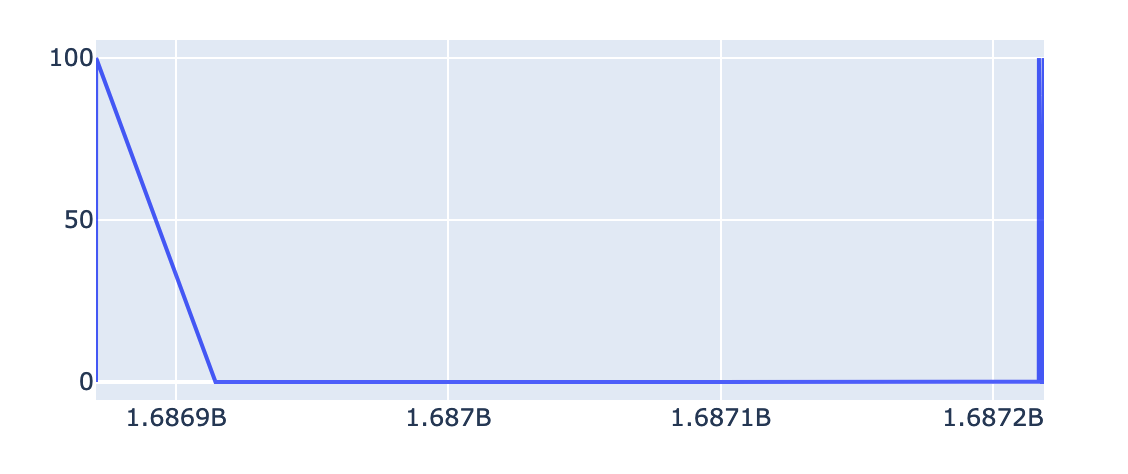
\includegraphics[width=3.125in, ]{jira_imgs/3920.png}

}
\begin{tabular}{p{2cm}p{14cm}}
\toprule
Step 7 & Step Execution Status: \textbf{ Pass } \\ \hline
\end{tabular}
 Description \\
{\footnotesize
Document the procedure including topics and time window. ~Particular
attention shall be paid to differences in interactions between the
running EFD and the archival version. ~If any topics chosen for this
test were downsampled in the archiving process, the document shall
report on the self consistency of the down/re-sampling of those topics.

}
\hdashrule[0.5ex]{\textwidth}{1pt}{3mm}
  Expected Result \\
{\footnotesize
\begin{itemize}
\tightlist
\item
  A document describing the process including the topics chosen and the
  time window.
\item
  The document shall be in the form of a notebook with saved outputs.
\end{itemize}

}
\hdashrule[0.5ex]{\textwidth}{1pt}{3mm}
  Actual Result \\
{\footnotesize
LVV-T2339.ipynb added to the DMTR-331 repo - also renderd at the end fo
the test report (\textbackslash secref\{sec:LVV-T2339nb\})\\
\strut \\

}




% This appendix is put in as part of the template. You may edit and add to it.
% It is not overwritten by Docsteady.

\newpage
\appendix
\section{Documentation}
The verification process is defined in \citeds{LSE-160}.
The use of Docsteady to format Jira information in various test and planing documents is
described in \citeds{DMTN-140} and practical commands are given in \citeds{DMTN-178}.

\section{Acronyms used in this document}\label{sec:acronyms}
\input{acronyms.tex}

\newpage

% Uncomment this if Docsteady makes you additional appendix
%% to be replaced by auto-generated file from docsteady (traceability appendix)


\end{document}
